\begin{figure}[ht]
    \centering{
    \begin{tikzpicture}
%    \draw (-7.8,-4.65)--(7.8,-4.65);
    
    % ROOT
    \node at (0,0) {\begin{minipage}{2in}\centering
        {\Large \underline{Dog Walker}}\\ Fig.~\ref{fig:dogwalker-protocol-PP}, Fig.~\ref{fig:dogwalker-protocol-PV}, and Fig.~\ref{fig:dogwalker-protocol-V}
    \end{minipage}};
        % L-CHILD (Rigidity)
        \node at (-3.25,-1) {$p_1+p_4$};
        \draw (0,-.5)--(-5,-1.75); 
        \node at (-5,-2.5) {\begin{minipage}{1.5in}\centering
            \underline{Rigidity Run}\\
            \RaggedRight
            Ensure $\pv$ behaves honestly
        \end{minipage}};
        
            % L-CHILD -- L-CHILD (Computation/Tomography)
            \node at (-6,-3.7) {$\frac{p_4}{p_1+p_4}$};
            \draw (-5,-3) -- (-5.85,-4.5);
            \node at (-5.85,-6.5) {\begin{minipage}{1.4in}\centering
                \underline{Computation Sub-run}\\ \underline{(Tomography)}\\
                \RaggedRight
                Ensure $\pv$ reports correct measurements when he gets to choose measurement to perform using $\textsc{tom}$ (Fig.~\ref{fig:tomography-test})
            \end{minipage}};
            
            % L-CHILD -- R-CHILD (Test/Clifford)
            \node at (-2.5,-3.7) {$\frac{p_1}{p_1+p_4}$};
            \draw (-5,-3) -- (-1.95,-4.5);
            \node at (-1.95,-5.775) {\begin{minipage}{1.4in}\centering
                \underline{Test Sub-run}\\ \underline{(Clifford)}\\
                \RaggedRight
                Ensure $\pv$ applies correct gates using $\textsc{rigid}$ (Fig.~\ref{fig:rigid})
            \end{minipage}};
        % R-CHILD (EPR)
        \node at (3.5,-1) {$p_2+p_3$};
        \draw (0,-.5)--(5,-1.75);
        \node at (5,-2.5) {\begin{minipage}{1.75in}\centering
            \underline{EPR Run}\\
            \RaggedRight
            $\pv$ uses EPR Protocol to delegate computation to $\pp$
        \end{minipage}};
        
            % R-CHILD -- L-CHILD (Computation)
            \node at (2.8,-3.7) {$\frac{p_2}{p_2+p_3}$};
            \draw (5,-3.2) -- (1.95,-4.5);
            \node at (1.95,-4.82)
            {\begin{minipage}{1.4in}\centering
                \underline{Test Sub-run}
            \end{minipage}};
                % R-CHILD -- R-CHILD -- L-CHILD (X-test)
                \node at (.6,-6) {$\sfrac{1}{2}$};
                \draw (1.95,-5.1) -- (0,-7);
                \node at (0,-8.5)
                {\begin{minipage}{1.4in}\centering
                    \underline{$X$-Test}\\           \RaggedRight
                    Ensure $\pp$ returns correctly measured bits, except for those returned on odd $\sf T$ gate gadgets
                \end{minipage}};
                % R-CHILD -- R-CHILD -- R-CHILD (Z-test)
                \node at (3.2,-6) {$\sfrac{1}{2}$};
                \draw (1.95,-5.1) -- (3.9,-7);
                \node at (3.9,-8.25)
                {\begin{minipage}{1.4in}\centering
                    \underline{$Z$-Test}\\           \RaggedRight
                    Ensure $\pp$ returns correctly measured bits on odd $\sf T$ gate gadgets
                \end{minipage}};
            % R-CHILD -- R-CHILD (Test)
            \node at (6,-3.7) {$\frac{p_3}{p_2+p_3}$};
            \draw (5,-3.2) -- (5.85,-4.5);            
            \node at (5.85,-5.05)
            {\begin{minipage}{1.4in}\centering
                \underline{Computation Sub-run}\\           \RaggedRight
                Run the computation
            \end{minipage}};
    \end{tikzpicture}}
    \caption{The structure of the Dog-Walker Protocol. We illustrate the structure of different runs, sub-runs, and games/tests, letting probabilities label branches.}
    \label{fig:DogWalkerFig}
\end{figure}